% !TEX TS-program = pdflatex
% !TEX encoding = UTF-8 Unicode

% This is a simple template for a LaTeX document using the "article" class.
% See "book", "report", "letter" for other types of document.

\documentclass[8pt]{article} % use larger type; default would be 10pt

\usepackage[utf8]{inputenc} % set input encoding (not needed with XeLaTeX)
\usepackage{bchart}
\usepackage{longtable}
\usepackage{pgfgantt}
\usepackage{calendar} % Use the calendar.sty style
\usepackage{calc}
\usepackage{ifthen}
\usepackage{tkz-base}
\usepackage{pdfpages}
\usepackage{hyperref}
\usepackage{pgfplots}
\usepackage{tkz-kiviat,numprint,fullpage} 
\usepackage{pgfplotstable} 
\usetikzlibrary{arrows}
\usepackage{paralist} % very flexible & customisable lists (eg. enumerate/itemize, etc.)
\usepackage{dcolumn}
\usepackage{booktabs}
\usepackage{lscape}
\usepackage{pgf-pie}
\usepackage{verbatim}
\usepackage{animate}
\usepackage{sfmath}

%%% Examples of Article customizations
% These packages are optional, depending whether you want the features they provide.
% See the LaTeX Companion or other references for full information.

\usepackage{textcomp}
%\usepackage{hyperref}

%%% PAGE DIMENSIONS
\usepackage{geometry} % to change the page dimensions
\geometry{a4paper} % or letterpaper (US) or a5paper or....
% \geometry{margin=2in} % for example, change the margins to 2 inches all round
% \geometry{landscape} % set up the page for landscape
%   read geometry.pdf for detailed page layout information

\usepackage{graphicx} % support the \includegraphics command and options

% \usepackage[parfill]{parskip} % Activate to begin paragraphs with an empty line rather than an indent

%%% PACKAGES
\usepackage{booktabs} % for much better looking tables
\usepackage{array} % for better arrays (eg matrices) in maths
\usepackage{paralist} % very flexible & customisable lists (eg. enumerate/itemize, etc.)
\usepackage{verbatim} % adds environment for commenting out blocks of text & for better verbatim
\usepackage{subfig} % make it possible to include more than one captioned figure/table in a single float
% These packages are all incorporated in the memoir class to one degree or another...

%%% HEADERS & FOOTERS
\usepackage{fancyhdr} % This should be set AFTER setting up the page geometry
\pagestyle{fancy} % options: empty , plain , fancy
\renewcommand{\headrulewidth}{0pt} % customise the layout...
\lhead{}\chead{}\rhead{}
\lfoot{}\cfoot{\thepage}\rfoot{}

%%% SECTION TITLE APPEARANCE
\usepackage{sectsty}
\allsectionsfont{\sffamily\mdseries\upshape} % (See the fntguide.pdf for font help)
% (This matches ConTeXt defaults)

%%% ToC (table of contents) APPEARANCE
\usepackage[nottoc,notlof,notlot]{tocbibind} % Put the bibliography in the ToC
\usepackage[titles,subfigure]{tocloft} % Alter the style of the Table of Contents
\renewcommand{\cftsecfont}{\rmfamily\mdseries\upshape}
\renewcommand{\cftsecpagefont}{\rmfamily\mdseries\upshape} % No bold!

%%% END Article customizations

%%% The "real" document content comes below...

%\includegraphics[width=.2\textwidth]{Logo.png}

\title{Finance}
\author{\copyright Frederic Kerdraon}
%\date{} % Activate to display a given date or no date (if empty),
         % otherwise the current date is printed 

%{\footnotesize
%Data are aggregated between Initial date: \textbf{2000-01-01} and Last date: \textbf{2018-11-16 00:00:00}

%}

%\addtobeamertemplate{frametitle}{}{%
%\begin{tikzpicture}[remember picture,overlay]
%\node[anchor=north west,yshift=2pt] at (current page.north west) {\includegraphics[height=0.8cm]{Logo1}};
%\end{tikzpicture}}

\begin{document}
\maketitle
\tableofcontents

\section{Stocks from Scilab}
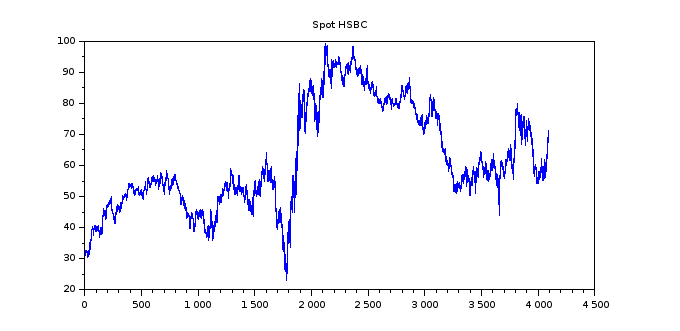
\includegraphics[scale=0.6]{Scilab-stocks.png}
This is the graph of HSBC stock 

%\section{Stocks from Qt}
%\includegraphics[scale=0.6]{Stockchart.png}

\subsubsection{Table}
Stocks results table is available in the database ;-)
Name, Standard deviation, VaR, Implied vol, ...
%\begin{longtable}{|c|c|c|c|c|}
\hline
\multicolumn{5}{|c|}{Cashflows} \\
\hline
Category & Debit & Credit & PnL \\
\hline
Other & 0.0000001 & 0.0000001 & 0\\
\hline
Other & 104 & 0 & -104\\
\hline
Other & 13 & 0 & -13\\
\hline
Other & 10 & 0 & -10\\
\hline
Other & 190 & 0 & -190\\
\hline
Other & 8 & 0 & -8\\
\hline
Other & 16 & 0 & -16\\
\hline
Other & 4 & 0 & -4\\
\hline
Other & 6 & 0 & -6\\
\hline
Other & 14 & 0 & -14\\
\hline
 ... & ... & ... & ...\\
\hline
 Total & 112143.00006290044 & 117930.00006290042 & 5786.99999999999 \\
\hline
\end{longtable}

\subsubsection{Analysis}
The graph is also available and produced by C++ under "legends"
%\includegraphics[width=.2\textwidth]{Legends.png}
%\begin{bchart}[min=0,max=11214,step=3738,unit=k\texteuro]
\bcbar[label=Other]{0}\\
\smallskip
\bcbar[label=Other]{10}\\
\smallskip
\bcbar[label=Other]{1}\\
\smallskip
\bcbar[label=Other]{1}\\
\smallskip
\bcbar[label=Other]{19}\\
\smallskip
\bcbar[label=Other]{0}\\
\smallskip
\bcbar[label=Other]{1}\\
\smallskip
\bcbar[label=Other]{0}\\
\smallskip
\bcbar[label=Other]{0}\\
\smallskip
\bcbar[label=Other]{1}\\
\smallskip
\end{bchart}

%\includepdf[pages={1}]{stockchart.pdf}

\end{document}

